\documentclass{article}
\usepackage[french]{babel}
\usepackage[utf8]{inputenc}
\usepackage[T1]{fontenc}
\usepackage{graphicx}
\usepackage{geometry}
\usepackage{caption}
\usepackage{subcaption}
\usepackage{listings}

\usepackage{courier}
\usepackage[colorlinks=true]{hyperref}
\hypersetup{
    linktoc=all,
    linkcolor=blue
}
\setlength{\parindent}{1cm}
\setlength{\textwidth}{15.5cm}
\setlength{\evensidemargin}{0.5cm}
\setlength{\oddsidemargin}{0.5cm}

\graphicspath{{tex/files/}}

\title{Rapport Projet S6 - FONCTIONNELLE}
\author{Romain PIERRE, Mathys MONELLO, Ilyes BECHOUAL, Yannis YOASSI PATIPE}
\date{Mai 2023}

\makeatletter
\let\mytitle\@title
\let\myauthor\@author
\let\mydate\@date
\makeatother

\begin{document}

\lstset{language=C, frame=single, basicstyle=\ttfamily, tabsize=4}

\begin{titlepage}
    \centering
    \vspace*{0.5 cm}
    
\includegraphics[width=5cm]{logo.jpg}\\[1.0 cm]
    \rule{\linewidth}{0.2 mm} \\[0.4 cm]
    \huge\textbf{\mytitle}\\
    \rule{\linewidth}{0.2 mm} \\[1.5 cm]  
    \LARGE\myauthor\\[1.0 cm]
    \large\textbf{\mydate}\\[2 cm]
    \begin{center}
        \huge
        "Tower Defense"
    \end{center}

    \vspace{4cm}
    \begin{center}
    EI6PR106 Projet de programmation fonctionnelle
    \\Département Informatique
    \\S6 - Année 2022/2023
    \end{center}
 \end{titlepage}

\tableofcontents

\newpage
\section{Introduction}
\textbf{Tower defense} est un jeu populaire dans lequel le but est d'empêcher les adversaires d'atteindre la ligne d'arrivée en utilisant des tours de défense. Ce semestre, nous avons entrepris la construction d'un jeu basé sur ce modèle, en mettant l'accent sur le paradigme de la programmation fonctionnelle en utilisant \textit{TypeScript}, une version avec syntaxe pour les types de \textit{JavaScript}. La programmation fonctionnelle est un paradigme dans lequel les expressions sont la base et sont combinées pour créer des expressions plus complexes. On y retrouve notamment les fonctions récursives, les fonctions de première classe et les fonctions anonymes. La difficulté de ce projet réside dans l'adoption d'une nouvelle méthode de pensée qui accompagne le paradigme fonctionnel. Cela peut sembler moins naturel que le paradigme impératif, surtout après avoir travaillé sur un projet en programmation impérative pendant un semestre. Cependant, la programmation fonctionnelle apporte une simplicité, une généralisation et une efficacité accrue. De plus elle permet de gagner beaucoup de temps sur certains points. Par exemple, l'indépendance des fonctions est particulièrement intéressant lors de modification, car elle évite de devoir changer l'intégralité du code.

\vspace{2cm}
\section{Compte-rendu}
Lors de ce projet, nous avons réalisé une interface graphique pour le terminal et une autre interface graphique pour une page web qui possède quelques fonctionnalités supplémentaires comme la possibilités d'afficher le tour suivant à la main par exemple. En ce qui concerne le jeu, nous avons implémenté un algorithme qui crée un chemin à l'aide de 4 points placés aléatoirement. Nous avons aussi créer plusieurs types d'attaquants, et nous avons décomposé chaque tour (que nous appellerons \textit{tick}) en 5 phases. 

\newpage
\section{Architecture du projet}
Cette section présente les choix d'architectures qui ont été fait pour ce projet.

\subsection{Dépendances}
Notre projet se décompose en 4 fichiers (or tests et fichiers de configuration). Le fichier \textbf{world.ts} gère tout ce qui est de la création du monde, sa génération aléatoire et ses spécificités (voir section \ref{world}). Le fichier \textbf{actor.ts} s'occupe de la création des différents acteurs de la partie et leurs fonctions associées (section \ref{actor}). Le fichier \textbf{engine.ts} quant à lui effectue la liaison entre les deux en proposant toutes les fonctions liées au jeu comme le spawn, les phases, l'affichage, etc (section \ref{engine}). Enfin \textbf{index.ts} est l'interface de notre projet et c'est depuis ce fichier que nous appelons toutes les fonctions.
\vspace{1cm}

La figure \ref{fig:depend} représente notre architecture. Les flèches symbolisent les dépendances entre les fichiers (\textit{i.e.} un import du fichier pointé). \textbf{index.ts} dépend naturellement de tous les autres fichiers. \textbf{world.ts} et \textbf{actor.ts} récupèrent tous deux les constantes définies dans \textbf{engine.ts} pour les identifiants des acteurs et des parcelles du monde. Enfin \textbf{engine.ts} hérite de la définition du type \textit{actor} pour le typage.
\vspace{1cm}

\begin{figure}[!h]
    \centering
    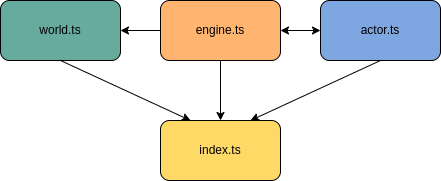
\includegraphics[width=13cm]{depend_js.drawio.png}
    \caption{Graphe des dépendances}
    \label{fig:depend}
\end{figure}

\newpage
\subsection{Programmation modulaire}
L’intérêt premier de ce choix d’architecture est d’avoir un code modulaire. En effet, en regroupant les sous-problèmes en fichiers distincts, il est plus facile de maintenir le projet ou l’améliorer. Il
suffit de respecter l’interface fixée et on peut ensuite travailler librement au sein même du fichier
sans altérer le reste du projet. De même, il n’est pas nécessaire d’avoir tous le projet en tête, et la
simple connaissance du fichier en question est suffisante pour travailler dessus.
Ainsi, la programmation modulaire facilite la modification du code et limite les bugs qui pourraient se généraliser à l’ensemble du projet, en contenant l’information au sein d’un même fichier. Il est
donc plus facile de se repérer et de collaborer.

\vspace{1cm}
\subsection{Programmation fonctionnelle}
Le code de ce projet \textit{TypeScript} devait donc respecter le paradigme de la programmation fonctionnelle au maximum. Pour se faire nous avons utilisé les techniques suivantes :
\vspace{0.5cm}

\begin{itemize}
\item La \textbf{récursivité} : La récursivité est une technique qui nous a permis d'améliorer la clarté de notre code (elle permet d'éliminer un bon nombre de boucles). De plus, cette approche est un peu plus naturelle pour la résolution de tâches répétitives.
\item Les \textbf{fonctions pures} : La pureté est une propriété très puissante. Les fonctions pures produisent un unique résultat pour une entrée donnée. De plus, elles sont indépendantes du reste du programme, ce qui apporte un certain contrôle sur les programmes et les tests.
\item L'\textbf{immutabilité} : L'immutabilité est une propriété très importante au niveau de la sécurité. Une variable immuable ne peut pas être modifiée après sa création, ce qui apporte de la sécurité au code et permet aussi de faciliter les tests.
%\item Les \textbf{fonctions internes} : 
\item Les \textbf{méthodes de haut niveau} : Ces méthodes sont parfaites pour l'abstraction. Elles permettent d'effectuer un nombre incalculable d'opérations sur des objets très complexes, ce qui simplifie grandement certains problèmes. Nous les avons beaucoup utilisé au cours de ce projet (notamment dans les fonctions de l'engine, section \ref{engine}).

\item Les \textbf{fonctions anonymes} : Les fonctions anonymes ont joué un rôle très important dans notre code. De par leur nature flexible et concise, elles nous ont permis de gagner en efficacité. Nous les avons souvent utilisé en tant que fonctions de première classe, notamment dans des méthodes de haut niveau telles que map, filter, etc. Cela nous a permis d'effectuer des opérations complexes sur des structures de données variées (tableaux d'objets, matrices, etc).

\end{itemize}
    
\newpage
\section{Création du monde}
\label{world}
Pour créer un \textbf{Tower Defense}, nous avons eu besoin de créer un monde sur lequel la partie peut se dérouler.
\subsection{Fonctionnalités}
Notre monde est implémenté par une matrice où les nombres représentent les identifiants des types de terrains et d'acteurs à chaque position. Nous avons décidé d'avoir un chemin principal en terre, qui part du point de départ des attaquants jusqu'à leur point d'arrivée. Ce chemin est accessible par tous les attaquants. Puis nous rajoutons une rivière qui elle n'est parcourable que par certains acteurs sachant nager. Ainsi selon le monde, certains attaquants pourront utiliser un raccourci pour arriver à leur fin. De plus, le monde stock l'emplacement des tours et des attaquants pour l'affichage et les phases de jeu.

\subsection{Algorithme de génération}
Pour créer notre monde, nous avons implémenté un algorithme de génération. Son fonctionnement est assez simple. On sélectionne aléatoirement 4 points du monde, le premier sur la première ligne qui sera le départ des attaquants, le deuxième et troisième sur deux lignes du milieu (respectivement à $1/3$ et $2/3$ de la hauteur) et le dernier sur la dernière ligne. Le dernier point représente la zone d'arrivée des attaquants. Ainsi une fois ces 4 points définis, il ne nous reste plus qu'à tracer les lignes entre en remplissant par le type de terrain que l'on souhaite. Pour ce faire, nous remplissons de proche en proche récursivement pour combler la plus grosse différence entre abscisse (dx) et ordonnée (dy) entre deux points. Ainsi notre algorithme fini forcément quand $dx=dy=0$. Nous avons choisi de tracer notre chemin principal comme ceci, puis de rajouter un cinquième point aléatoirement sur une ligne centrale et tracer de même la rivière accessible qu'à certains acteurs entre le deuxième, le cinquième et le quatrième point. La figure \ref{mondeexemple} montre quelques exemples d'exécution de notre fonction:
\textit{createWorld()}. 
\vspace{1cm}

\begin{figure}[!h]
    \centering
    \begin{subfigure}{0.3\textwidth}
    \centering
        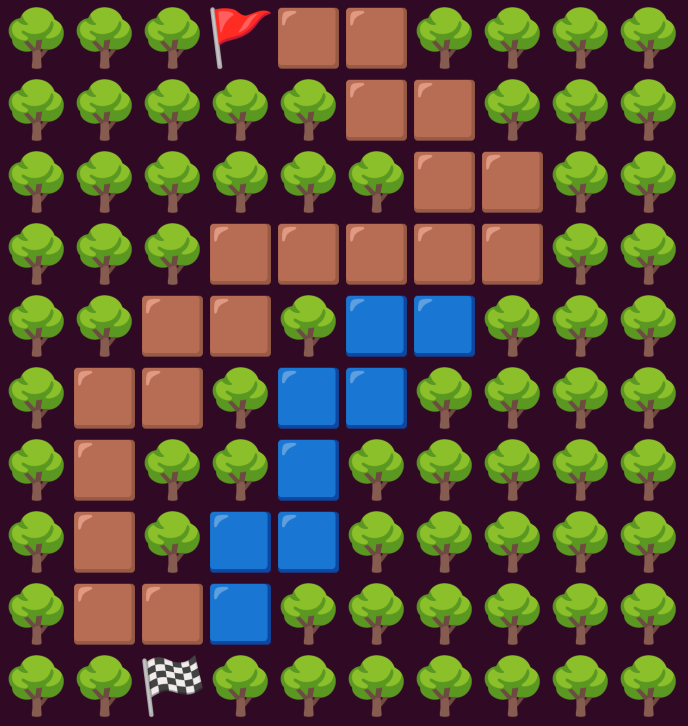
\includegraphics[width=\textwidth]{world1.png}
    \end{subfigure}
    \hfill
    \begin{subfigure}{0.3\textwidth}
        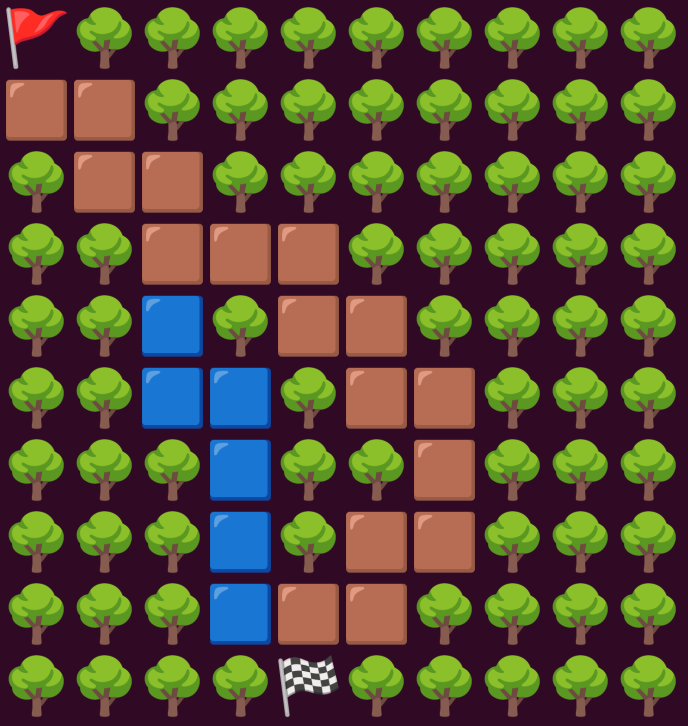
\includegraphics[width=\textwidth]{world2.png}
    \end{subfigure}
    \hfill
    \begin{subfigure}{0.3\textwidth}
        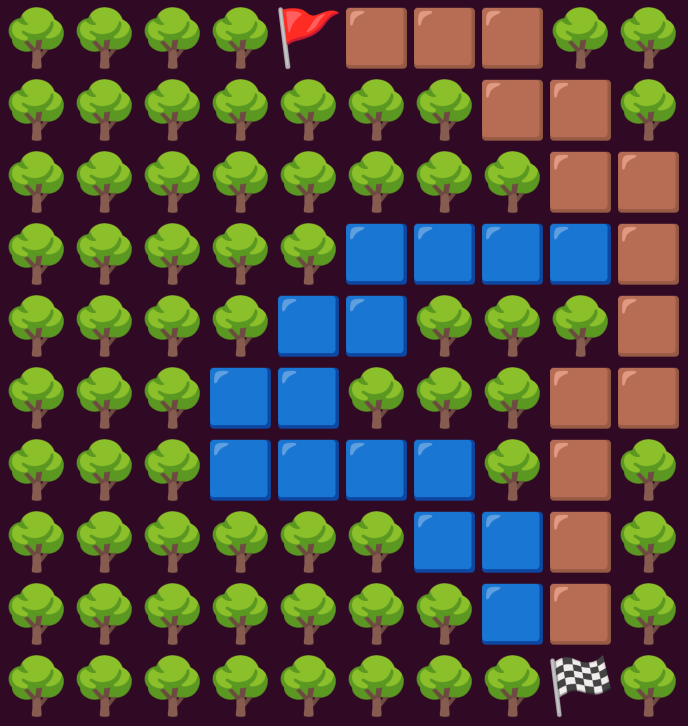
\includegraphics[width=\textwidth]{world3.png}
    \end{subfigure}
    \caption{Exemples de mondes construit aléatoirement (ici en 10x10)}
    \label{mondeexemple}
\end{figure}

\newpage
\section{Acteurs de la partie}
\label{actor}
Notre jeu contient deux catégories d'acteur, des \textbf{défenseurs} et des \textbf{attaquants}. Ils se battent entre eux afin de réaliser leur objectif. Les acteurs que nous avons implémenté diffèrent simplement par leurs statistiques et le fait qu'il soient statiques ou non.
\subsection{Défense}
Nous n'avons réalisé qu'un défenseur: \textbf{une tour}. Cet acteur est donc un acteur immobile qui apparaît sur le monde mais toujours collé à un chemin, que ce soit le chemin terrestre ou la rivière. Les tours apparaissent selon une période fixe. Cette période est de 20 ticks. Ce sont des acteurs à qui nous avons décidé d'accorder beaucoup de points de vie par rapport aux attaquants, afin de compenser le fait qu'ils sont moins nombreux et qu'ils ne se déplacent pas. Nous leur avons assigné une zone d'attaque circulaire qui regroupe plusieurs cases afin de simuler une tour avec des archers. Ces tours infligent peu de dégâts par rapport aux attaquants afin d'équilibrer le jeu car les attaquants possèdent moins de points de vie et reçoivent des dégâts sur plusieurs cases. De plus ils peuvent être bloqués sur une case lors de la phase \textit{blocage} ce qui permet aux défenseurs de leur infliger plus de dégâts.

\subsection{Attaque}
Les attaquants apparaissent tous les 10 ticks, ils sont au nombre de 3, chacun avec des caractéristiques et des probabilités d'apparition différentes :\\

\begin{itemize}
\item Les \textbf{attackers} : Ce sont les attaquants par défaut, ils se déplacent en majorité uniquement sur le chemin terrestre, mais certains sont capables de nager et donc de se déplacer en empruntant la rivière (avec une probabilité de 1/3). Grâce à leur très grande probabilité d'apparition, ils permettent d'avoir des parties avec bon nombre d'acteurs, par contre, ils ont relativement peu de vie, ce qui en fait des acteurs vulnérables.\\

\item Les \textbf{megAttackers} : Ce sont des attaquants qui possèdent beaucoup plus de points de vie (presque le même nombre qu'une tour) que les attaquants par défaut, mais ils sont incapable de nager. Ceux-ci garantissent la victoire des attaquants en beaucoup moins de tours, c'est d'ailleurs pour cela qu'ils ont une probabilité d'apparition de 1/10 (sachant qu'un attaquant apparaît tous les 10 ticks).\\

\item Les \textbf{speedAttackers} : Ce sont aussi des attaquants améliorés. Comme les megAttackers, ils ne peuvent pas nager et ont une probabilité d'apparition plus faible (1/10 tous les 10 tours). Les speedAttackers se déplacent beaucoup plus vite (de deux cases en deux cases).\\
\end{itemize}

Avoir plusieurs attaquants est un choix que nous avons fait, afin de permettre d'avoir des parties variées.
\newpage
\section{Moteur du jeu}
Dans cette partie, nous allons présenter comment nous avons gérer le monde, les acteurs et les phases de jeu.
\label{engine}

\subsection{Gestion du monde et des acteurs}
Pour gérer notre monde, nous avons décidé d'utiliser une matrice dans laquelle nous initialisons les coefficients pour les faire correspondre à des éléments du monde et ainsi, différencier les différentes entités qui le compose. Les correspondances entre entier et entité sont définies à l'aide du type \textit{type} dans lequel nous assignons une valeur à une entité spécifique.
\\Ensuite pour les acteurs, nous avons créé un type \textit{actor} générique dans lequel nous avons définis les caractéristiques et les actions que contiennent les acteurs. À l'aide de ce type, nous avons ensuite créer deux fonctions distinctes pour initialiser les attaquants et les défenseurs. Ces deux fonctions permettent de définir les statistiques des attaquants et des défenseurs de base, ainsi que leurs fonctions associées. En ce qui concerne les "supers" attaquants, pour les créer, nous utilisons la fonction pour créer un attaquant puis nous changeons ses statistiques et sa représentation graphique à l'aide d'une autre fonction. Cette façon de faire permet de ne pas créer plusieurs fonctions pour créer différents attaquants. Cela simplifie grandement la tâche et augmente la flexibilité de notre code.
\subsection{Gestion des phases de jeu}
Pour la gestion des phases de jeu, nous avons décidé d'établir un prototype universel pour les fonctions prenant part à la boucle. Le prototype est le suivant: \\\textit{nom\_de\_la\_fonction(actor : Actor.actor, actorArray : Actor.actor[], world : number[][]) : number}.
\\Ce prototype nous permet d'utiliser les fonctions tour à tour à l'aide du tableau \textit{action} qui les regroupe. Il nous permet aussi d'utiliser tous les paramètres dont nous avons besoin pour utiliser les phases que nous avons implémenté dans un appel uniforme.
\\Nous avons décidé d'implémenter les phases suivantes: 
\begin{itemize}
    \item \textbf{Mouvement}
    \item \textbf{Attaque}
    \item \textbf{Soin}    
    \item \textbf{Esquive}
    \item \textbf{Blocage}
\end{itemize}


Certaines phases sont propres aux attaquants et d'autres aux défenseurs car la tour ne peut pas esquiver une attaque par exemple à cause de son immobilité. Dans ce cas l'acteur renvoi un retour neutre à l'appel de l'action (exemple: la tour retourne dx: 0, dy: 0 pour le mouvement). Les phases de \textit{mouvement}, d'\textit{attaque} et de \textit{soin} sont des évènements récurrents de la partie car elles se produisent à chaque tour. Les acteurs attaquent dès qu'ils peuvent et se soignent lorsqu'ils ne sont plus en combat. Contrairement à la phase d'\textit{esquive} ou de \textit{blocage} qui s'activent aléatoirement lors d'un combat. Dans le but de simuler l'esquive, nous avons décidé de rajouter avant le coup, les points de vie que va perdre l'attaquant, afin d'éviter de le faire mourir s'il n'a pas assez de vie. Nous aurions aussi pu changer les points d'attaque de la tour en les mettant à 0, mais cela impliquerait qu'on devrait changer une nouvelle fois les points d'attaque de la tour pour les remettre à leur valeur initiale. Aussi, cela impliquerait que tous les attaquants esquiveraient en même temps, ce qui ne rendrait pas les attaquants comme des personnages distincts mais plutôt comme un groupe. Ce qui n'est pas intéressant pour l'équilibrage du jeu.

\newpage
\section{Spécification du jeu}
\noindent Le jeu se présente de cette façon :\\
\begin{itemize}
    \item Un monde rectangulaire est créé, avec un chemin de terre et d'eau reliant les points de départ et d'arrivée, générés aléatoirement de haut en bas.\\
    \item Il existe des acteurs attaquants et défenseurs. Les attaquants apparaissent tous les 10 tours, alors que les défenseurs apparaissent tous les 20 tours.\\
    \item Les attaquants peuvent se déplacer exclusivement sur les chemins de terre ou d'eau. Tandis que les défenseurs doivent être à l'extérieur de ces chemins.\\
    \item Le jeu comprend cinq phases de jeu, qui sont organisées de la manière suivante : la phase de mouvement, où seuls les attaquants peuvent se déplacer ; la phase d'attaque, où à la fois les attaquants et les défenseurs peuvent effectuer des attaques ; la phase de soin, où les attaquants et les défenseurs peuvent se soigner ; la phase d'esquive, réservée aux attaquants pour esquiver les attaques ; et enfin la phase de blocage, qui est déclenchée par les tours de défense et vise à bloquer les attaques ennemies.\\ 
    \item Il ne peut y avoir plusieurs acteurs sur une même position.\\
    \item L'objectif des attaquants est d'arriver sur la ligne d'arrivée, tandis que celui des défenseurs est de les en empêcher. À chaque fois qu'un attaquant atteint la ligne d'arrivée, le joueur perd une vie. Le jeu s'arrête lorsque le joueur n'a plus de points de vies.\\
    \item Les attaquants apparaissent sur la ligne de départ. Il y a 4 types d'acteurs : un acteur simple, un acteur simple pouvant nager et pouvant ainsi emprunter le chemin d'eau, un type de super attaquant qui a plus de vie et d'attaque, et un attaquant rapide.\\
    \item Les défenseurs, qui se présentent sous forme de tours, sont plus puissants que les attaquants mais sont moins nombreux. Ils apparaissent aléatoirement près des chemins de terre ou d'eau.
\end{itemize}

\newpage
\section{Affichages}
Cette partie présente les affichages de notre jeu.

\subsection{Console}
    L'affichage se fait lors de chaque tour de la partie comme le montre la figure \ref{fig:terminal}, en effectuant des \textbf{console.log()}. Les éléments affichés sont le nombre actuel d'attaquants, leurs points de vie, les points de vie des tours, le numéro du tour du jeu et l'ordre d'exécution des phases. L'affichage du plateau de jeu se fait également avec un \textbf{console.log()}, mais en parcourant la matrice avec une méthode \textbf{.map()}. Cette façon de faire est impure car l'affichage produit des effets de bord, mais il est important d'afficher pour avoir l'état de la partie en temps réel lors des phases de débug par exemple.
\begin{figure}[!h]
    \centering
    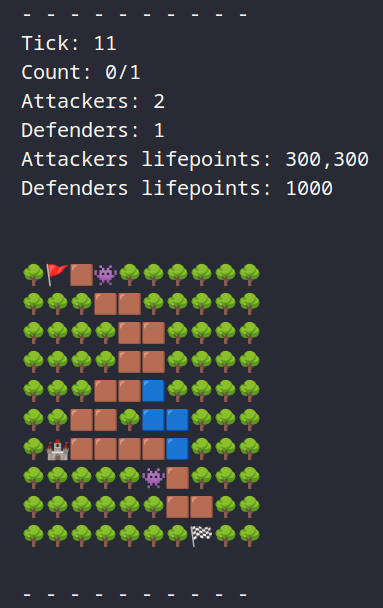
\includegraphics[width=4.5cm]{terminal.png}
    \caption{Affichage sur la console avec un monde de taille 10 x 10.}
    \label{fig:terminal}
\end{figure}
\subsection{HTML}
   La partie \textit{HTML} a été complexe en raison de notre inexpérience en \textit{HTML}, \textit{CSS} et de leur association avec \textit{JavaScript}. Toutefois, l'utilisation de Parcel, un outil intéressant pour la création de sites web avec ces trois langages, a grandement facilité la tâche. Après avoir appris certaines notions de base du langage, nous avons cherché à afficher la partie. C'est alors qu'un problème est survenu l'affichage étant fait dans la boucle de jeu. La conclusion a été que la boucle de jeu devait être modifiée afin qu'elle n'exécute qu'un seul \textbf{tick} à chaque appel. Ainsi, différents affichages ont été réalisés sans répéter de code et un niveau de \textit{Tower Defense} spécial non-violent a même été créé, où le but est de pêcher le plus de poissons possibles (voir l'annexe \ref{fig:lvl1}). Il y a deux méthodes d'arrêt du jeu. La première est de perdre tous ses coeurs et donc de perdre la partie. La seconde est de cliquer sur le bouton rouge \textbf{Stop Game} comme on peut le voir dans la Figure \ref{fig:buttonHTML}. D'autres éléments sont affichés de la même manière que pour l'affichage console.

\subsubsection{Fonctions asynchrones}
    Ce choix a été fait initialement pour l'affichage sur le terminal, permettant de visualiser l'évolution de la partie de manière progressive à l'aide de la fonction \textbf{setTimeout()}, qui met en file d'attente l'exécution d'une fonction. Bien que ce choix puisse être critiqué car il contient des effets de bord, ce qui est contraire à la programmation fonctionnelle, nous avons préféré la praticité qu'offre l'asynchronicité. De plus, cela a également aidé pour l'affichage de l'\textit{HTML}, car celui-ci utilise une promesse de clic et n'exécute un \textbf{tick} que s'il y a un clic sur le bouton \textit{next turn} comme décrit sur l'image \ref{fig:random_html}. On peut noter qu'il y des cases blanches avec un cercle rouge cliquables, qui font apparaître des tours si l'on a assez de tours restantes dans le stock de tour.

\begin{figure}[!h]
    \centering
    \begin{subfigure}{0.6\textwidth}
    	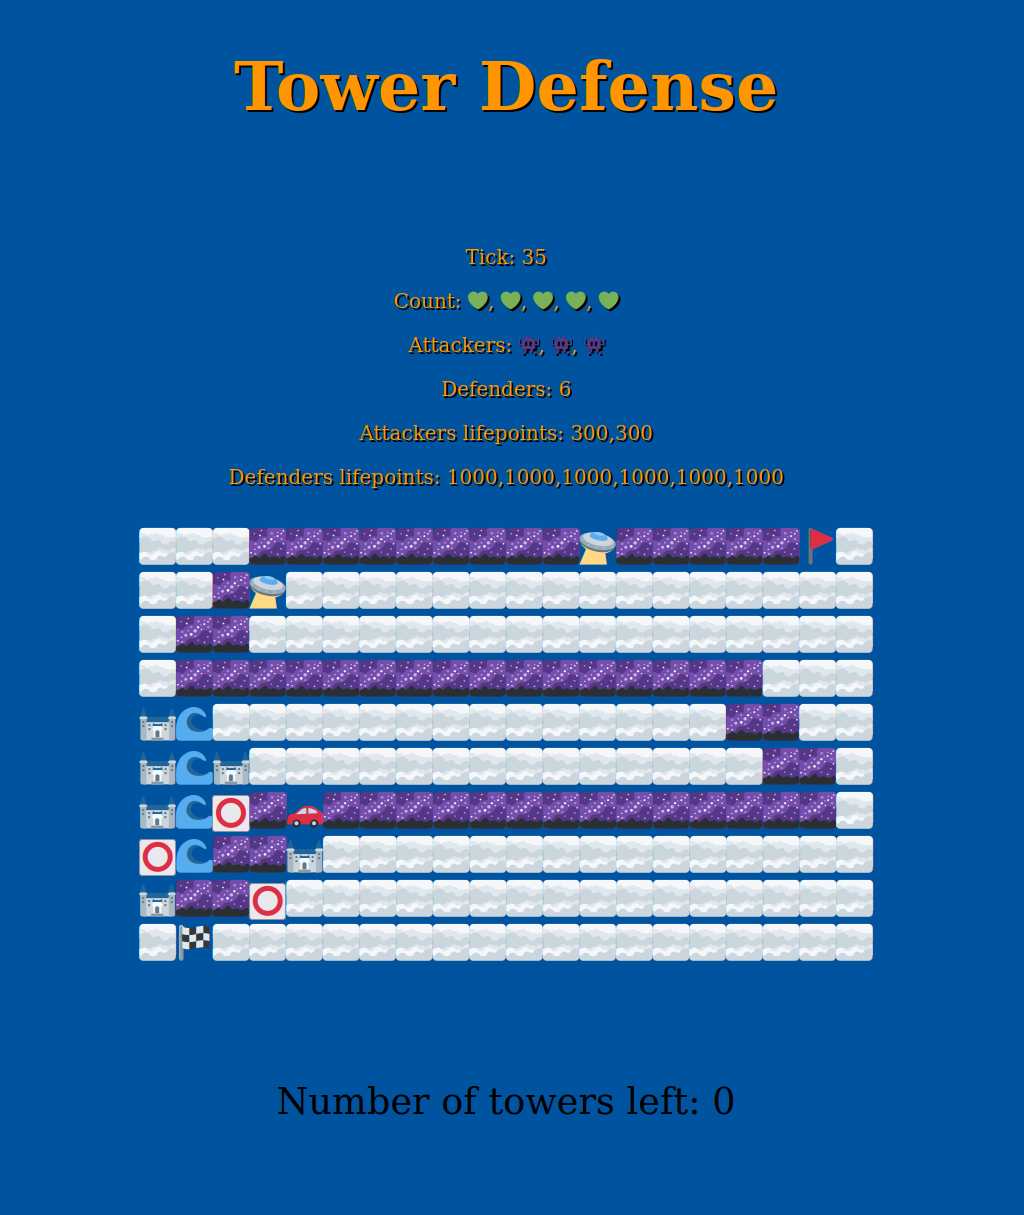
\includegraphics[width=\textwidth]{TowerDRandom.png}
   	 \caption{Partie avec la génération aléatoire de taille 20 x 10.}
	    \label{fig:random_html}
    \end{subfigure}
    \hfill
    \begin{subfigure}{0.6\textwidth}
        
\includegraphics[width=\textwidth]{buttonHTML.png}
    	\caption{Bouton de jeu HTML.}
            \label{fig:buttonHTML}
    \end{subfigure}
\end{figure}


\newpage
\section{Tests unitaires}
En ce qui concerne les tests, nous avons testé nos fonctions à l'aide de \textbf{Jest} par fichier, en prenant soin de vérifier qu'elles réalisent bien ce que l'on souhaite. Cela nous permet d'identifier plus rapidement la partie de la fonction qui pose problème, puisque les fonctions d'un fichier vont dépendre d'un autre. Nous avons une couverture de test de minimum 80\% par fichier. Les 20\% restant étant les fonctionnalités les moins importantes.

\vspace{1cm}
\section{Outils de travail}
Lors de ce projet, nous avons découvert de nouveaux outils. En effet, puisque c'est le premier projet que nous réalisons en \textit{Typescript} et pour lequel, on nous demande de créer une interface web, c'est-à-dire qui nécessite l'utilisation d' \textit{HTML} et de \textit{CSS}. Nous avons aussi pu approfondir notre utilisation du module \textbf{Jest} qui permet de faire des tests de manière simplifiée. Cela nous a permis de découvrir le module \textbf{Mock} lors de la réalisation de nos tests, qui permet de reproduire ou remplacer une fonction afin de déterminer à l'avance la valeur que la fonction qui est remplacée va renvoyer. Nous avons aussi eu l'occasion de continuer à améliorer notre utilisation de \textit{git} et des possibilités qu'il présente. Ainsi, nous n'avons pas hésité à créer une branche lorsqu'on devait implémenter la partie HTML. L'utilisation de cette branche nous a permis de continuer à développer le projet en pouvant publier notre avancée sur la forge, sans que cela affecte le code principal.
\vspace{1cm}

\section*{Conclusion}
    Ce projet nous a montré une nouvelle façon de coder et de réfléchir à un problème donné. Dans un premier temps, nous ne comprenions pas l'intérêt de coder uniquement en fonctionnel. De plus, le sujet initial qui est l'implémentation du jeu \textbf{Tower Defense}, se base généralement sur une boucle, ce qui est loin d'être fonctionnel. Mais le réel objectif derrière tout cela est de nous donner plus de champ de résolution lorsque nous sommes confronté à un certain problème. Il s'agit de rendre nos fonctions aussi génériques et réutilisables que possible, ce qui facilite la maintenance et l'extension du code à long terme. En effet, en utilisant des fonctions pures et des concepts tels que la composition de fonctions, nous pouvons écrire des fonctions qui résolvent des problèmes spécifiques de manière générique, ce qui nous permet de les réutiliser dans d'autres parties de notre code.\\
    De plus, l'utilisation de \textit{Typescript} est plus qu'adaptée pour un projet de groupe, car elle apporte de l'uniformité dans les objets dont on parle et que l'on manipule. Hormis la phase d'adaptation, le projet n'a pas causé de grandes difficultés, car la répartition des tâches et la mise en place d'une convention sur notre manière de nommer et de coder nous a grandement aidé dans la réalisation du projet.

\newpage
\section{Annexe}
\begin{figure}[!h]
    \centering
    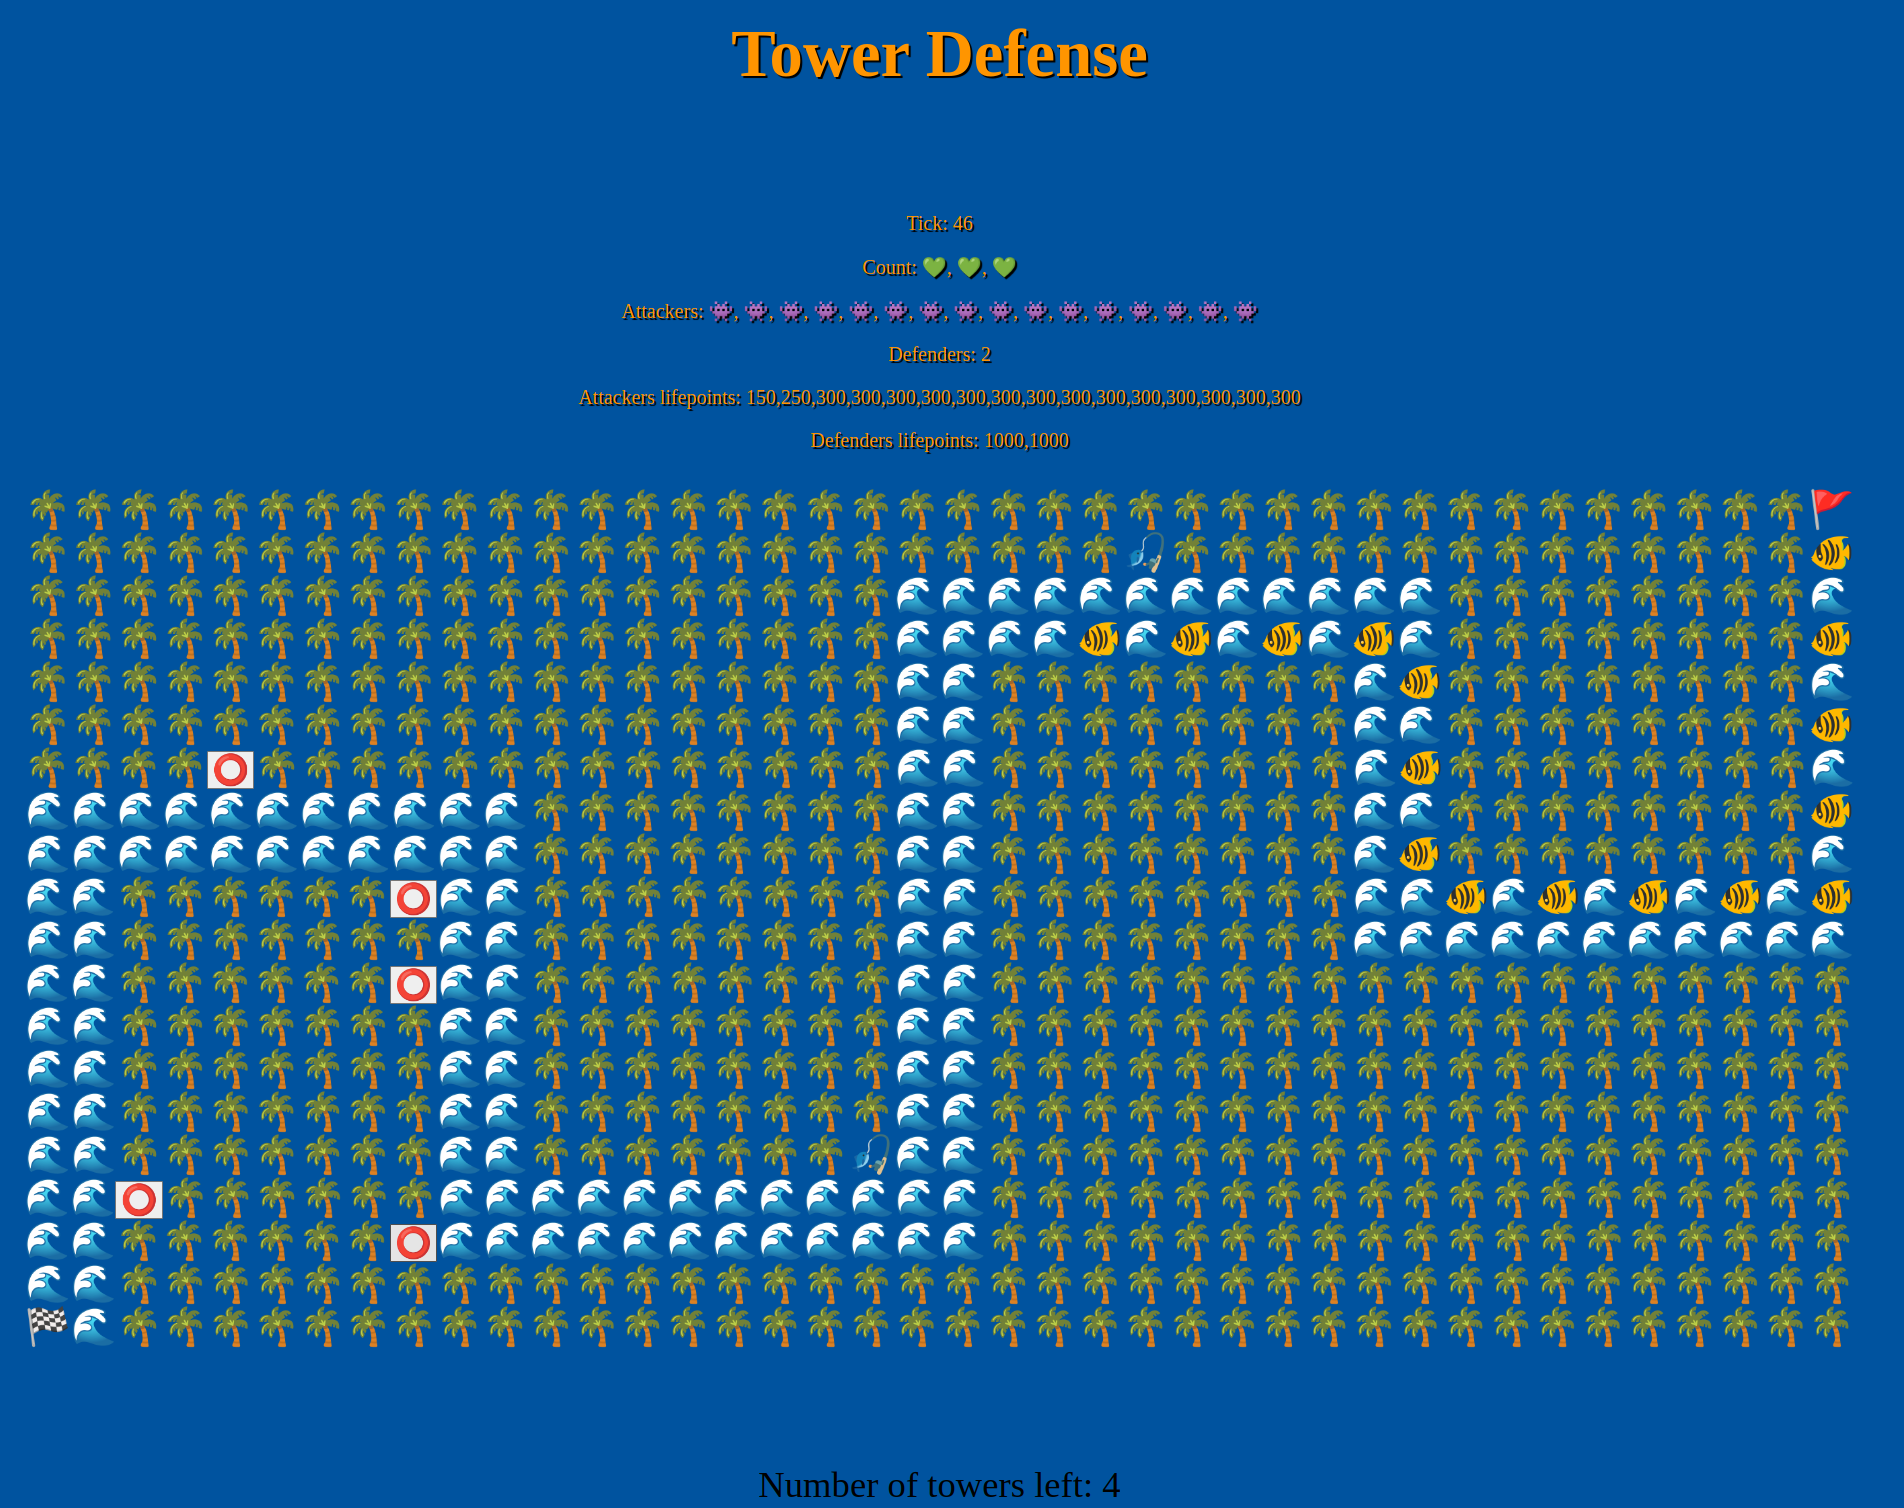
\includegraphics[width=15cm]{HTML_Lvl1.png}
    \caption{Le niveau 1 de Tower Defense}
    \label{fig:lvl1}
\end{figure}

\end{document}
